\section{Overall description}
\label{sect:overalldescription}

%\begin{sidewaysfigure}
%\centering
%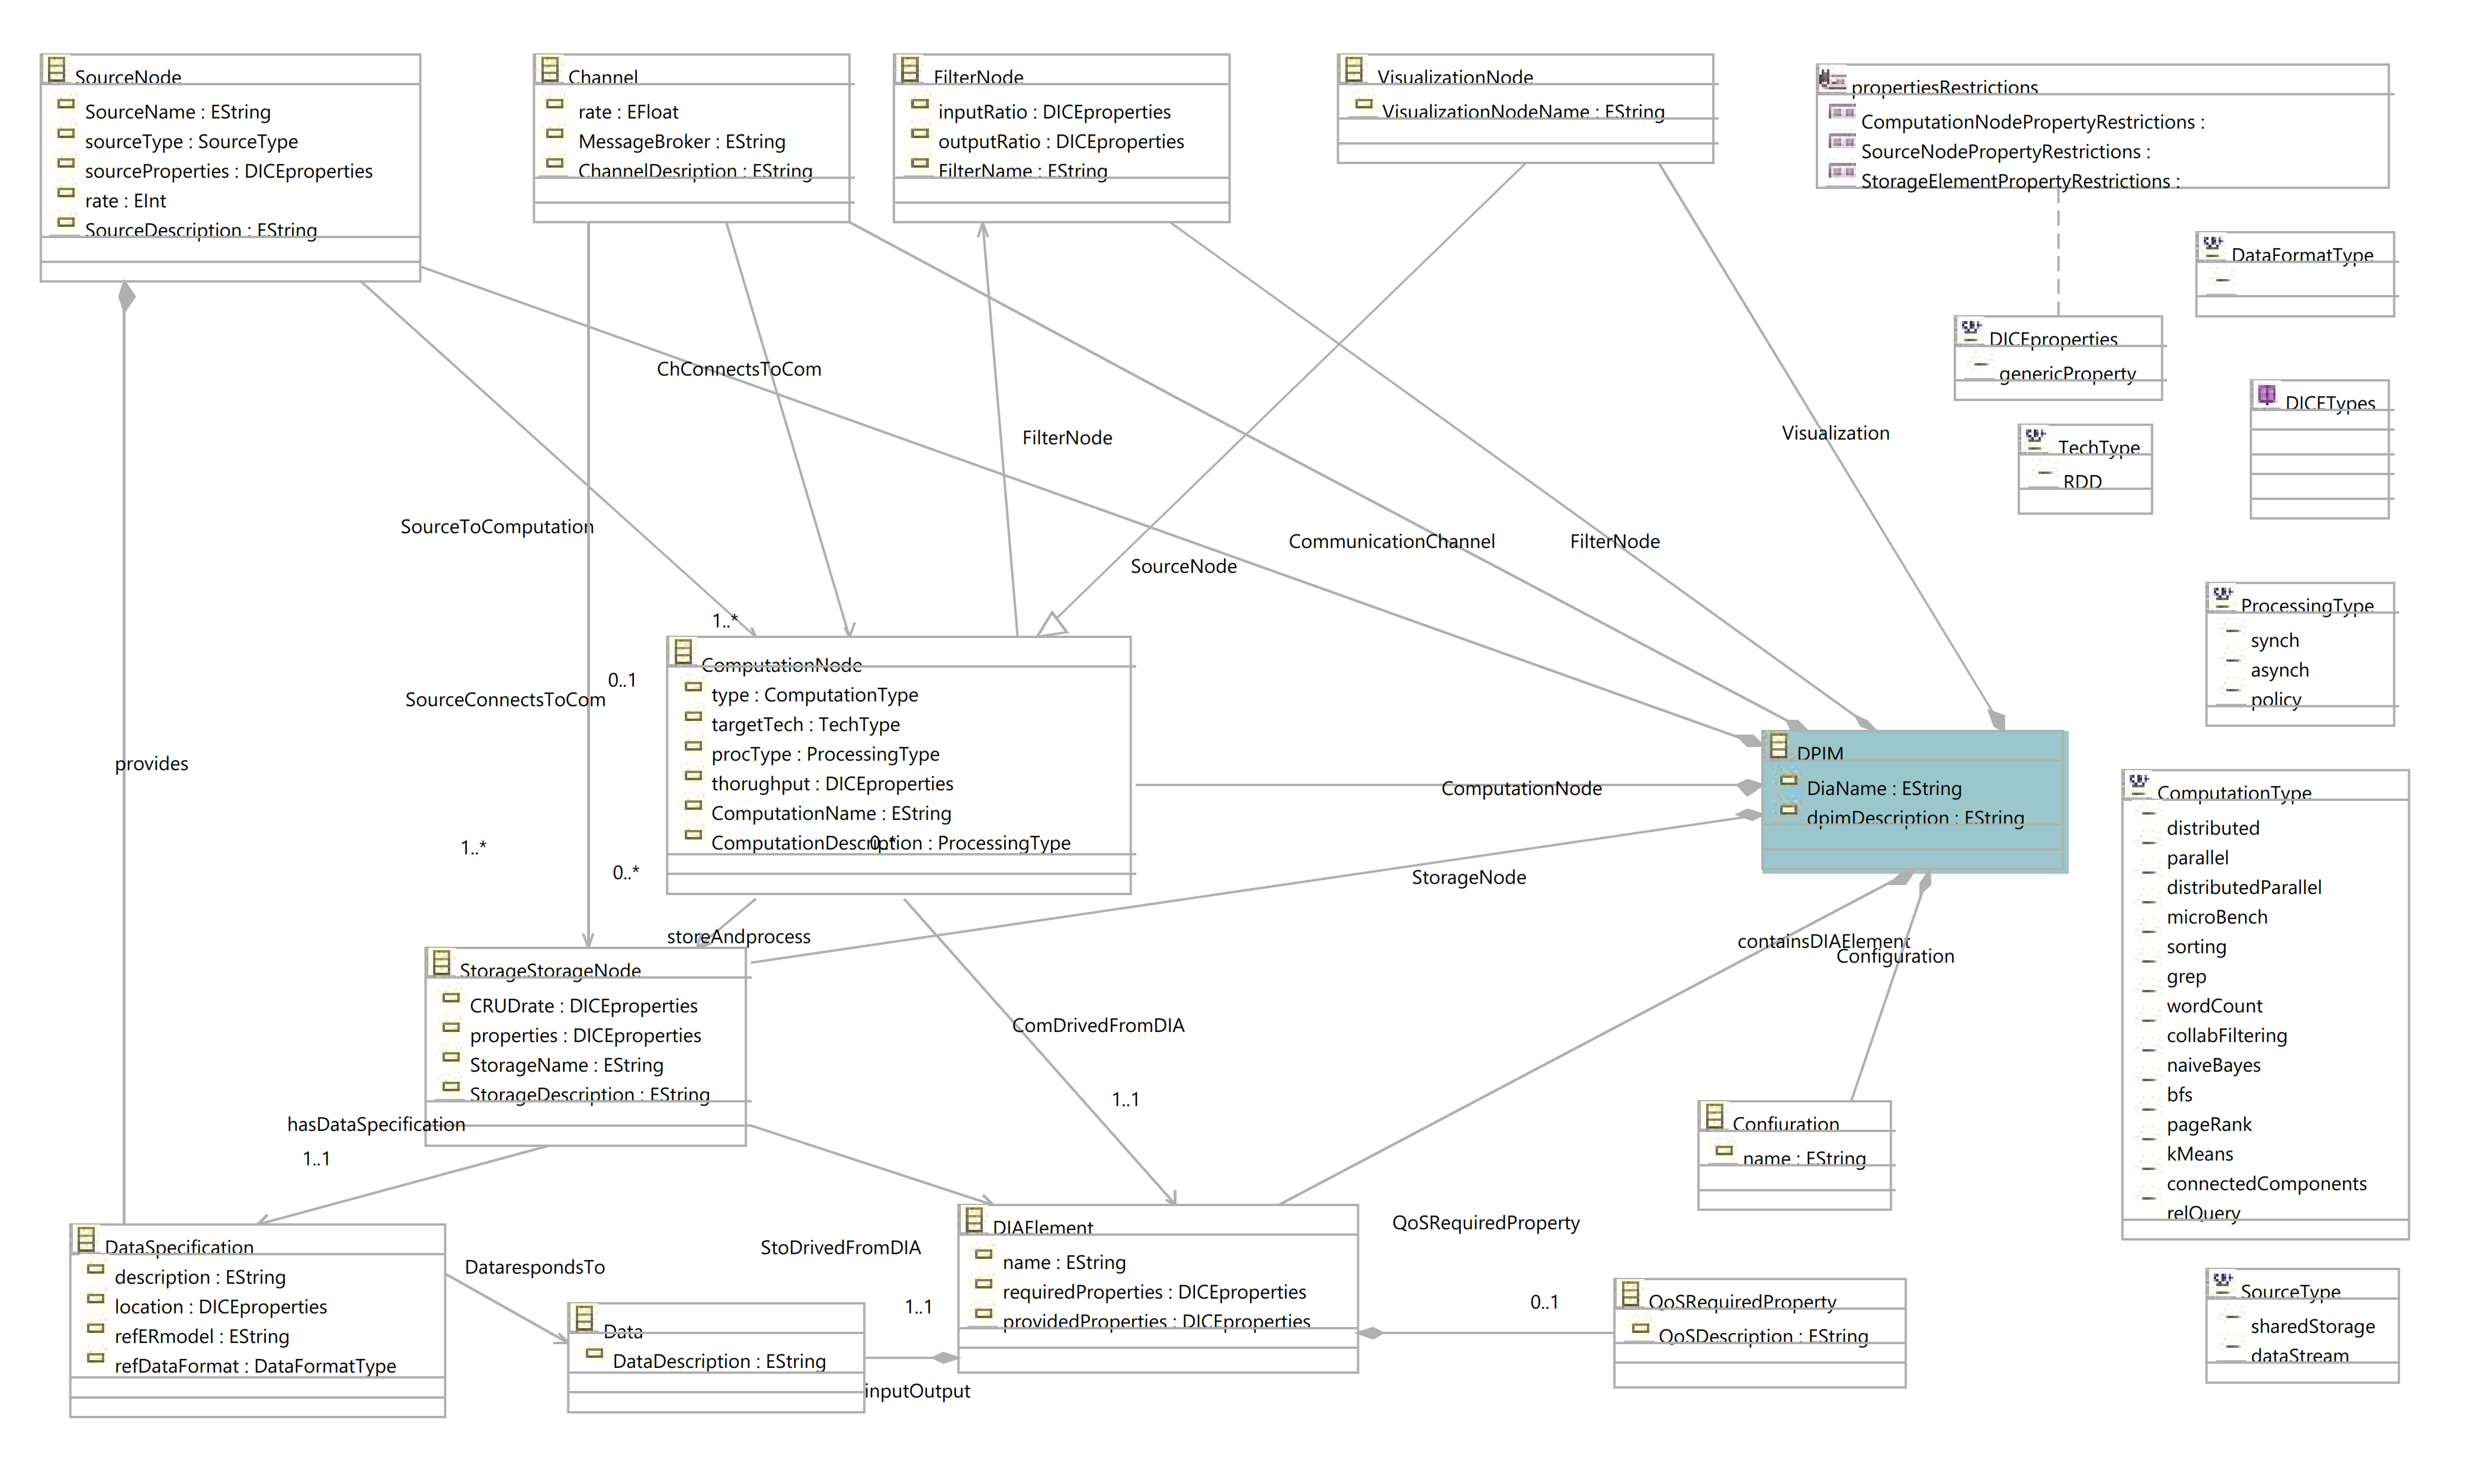
\includegraphics[width=\textwidth]{Images/11.png}
%\caption{\label{fig:metamodel}DICE DPIM metamodel.}
%\end{sidewaysfigure}

%\begin{figure}
%\centering
%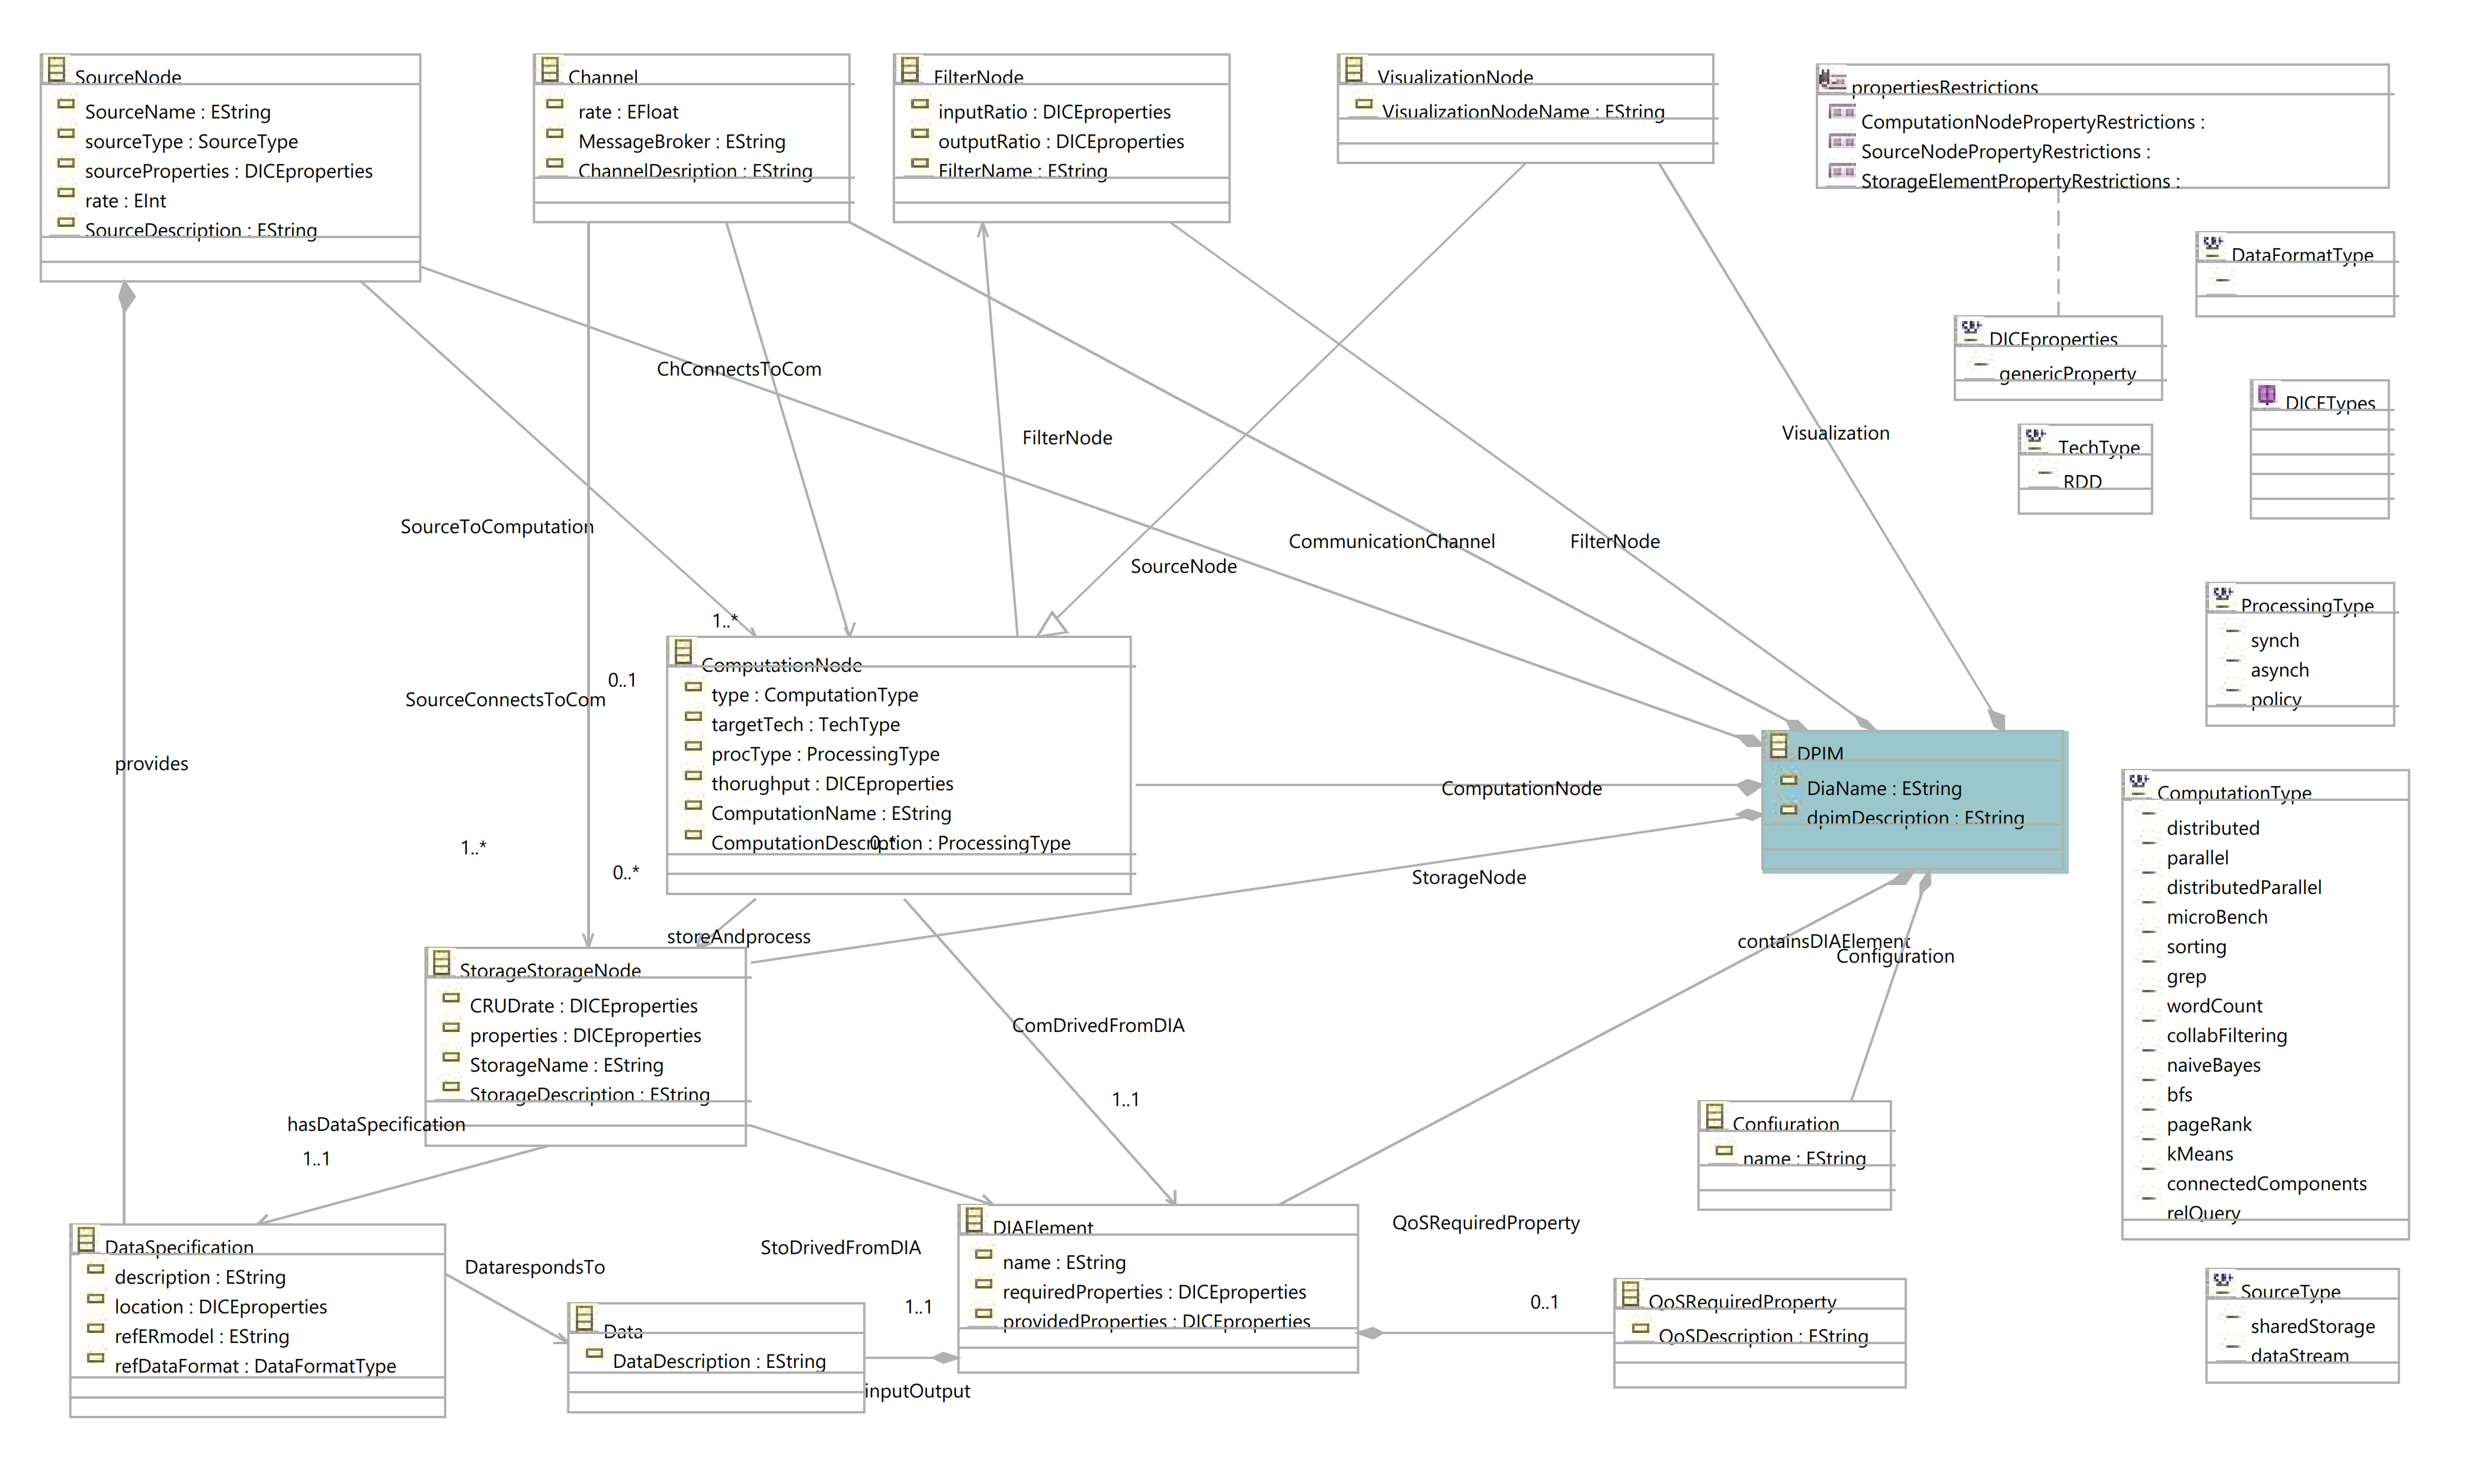
\includegraphics[width=\textwidth]{Images/11.png}
%\caption{\label{fig:metamodel2}DICE DPIM metamodel in portrait form.}
%\end{figure}

\subsection{Goals}
\label{subsect:goals}

The following table shows in details all the main goals that our application wants to meet. 

We managed to divide them in two main categories: goals related to the shop owners and goals related to the clients. Also, we have assigned an unique identifier to each one of them in order to be able to refer to them later in the document.

\begin{table}[h!]
    \centering
    \begin{tabular}{@{}P{0.1\textwidth}P{0.80\textwidth}@{}}
        \multicolumn{2}{c}{\textbf{Shop owners}} \\
        \toprule
        \textbf{Identifier}& \textbf{Goal}\\
        \midrule
        \textbf{G1}        & Allow manager to sign on the system\\
        \textbf{G2}        & Allow a manager to sign in the system\\
        \textbf{G3}        & Allow a manager to register their store/stores on the system\\
        $\;\;$    G3.1  & Allow a manager to register basic info about the shop\\
        $\;\;$    G3.2  & Allow a manager to divide their store in areas \\
        $\;\;$    G3.3  & Allow a manager to register the items in the areas \\
        \textbf{G4}        & Allow a manager to update the shop info\\
        \textbf{G5}        & Allow a manager to check the general status of their shop\\
        \textbf{G6}       & Allow a manager to cancel a previously booked shopping session for a user \\

    \end{tabular}
\caption{Shop owner's goals}
\label{table:shopownersgoals}
\end{table}

\begin{table}[h!]
    \centering
    \begin{tabular}{@{}P{0.1\textwidth}P{0.80\textwidth}@{}}
        \multicolumn{2}{c}{\textbf{Clients}} \\
        \toprule
        \textbf{Identifier}& \textbf{Goal}\\
        \midrule
        \textbf{G7}        & Allow a customer to join the virtual queue from the spot\footnotemark\\
        \textbf{G8}        & Allow a user to sign on the system\\
        \textbf{G9}        & Allow a user to sign in the system\\
        \textbf{G10}        & Allow a user to join the virtual queue from the app\\
        \textbf{G11}       & Allow a user to book a shopping session at a grocery store\\
        $\;\;$    G11.1 & Allow a user to select the time and duration(between predefined options) for they session\\ 	
        $\;\;$    G11.2 & Allow a user to select categories of items they are willing to buy\\
        \textbf{G12}       & Allow a user to retrieve informations about its previously booked visits\\
        \textbf{G13}       & Allow a user to retrieve informations about the congestion of shops\\
        \textbf{G14}       & Allow a customer to use a QR code to get access to the store \\
        \textbf{G15}       & Allow a customer to exit a previously joined queue \\
        \textbf{G16}       & Allow a customer to cancel a previously booked shopping session \\

        \bottomrule
    \end{tabular}
\caption{Client's goals}
\label{table:clientsgoals}
\end{table}
\footnotetext{with the facility of a hardware support, it will be better specificed later on this document.}

\subsection{Domain Assumptions}
\label{subsect:domainassumptions}

The following table list all the assumptions over which we cannot have control, but we assume as verified.

As with the goals in the section above, we provide them with an unique identifier to keep track of them in the document.

\begin{table}[h!]
    \centering
    \begin{tabular}{@{}P{0.1\textwidth}P{0.80\textwidth}@{}}
        \toprule
        \textbf{identifier}& \textbf{Domain Assumption}\\
        \midrule
        \textbf{D1}        & Data provided from GPS is valid and accurate\\
        \textbf{D2}        & Google Maps' paths calculator makes correct time estimations\\
        \textbf{D3}        & A person cannot get in the store without having scanned the QR code\\
        \textbf{D4}        & A person cannot get out of the store without having scanned the QR code\\
        \textbf{D5}        & The number of people entering the store is coherent with the data related to the QR code scanned\\
        \textbf{D6}        & Each store registered on the system is provided with the necessary functioning hardware\\
        \textbf{D7}        & Data provided from managers is legit\\
        $\;\;$D7.1         & Managers provide the maximum number of person allowed in the store by the law (non penso sia da mettere, non è di nostro interesse che questo dato sia corretto secondo la legge. L'unica cosa che ci interessa è che questo dato venga inserito per forza, e possiamo occuparcene obbligando il manager a scriverlo al momento della registrazione del negozio)\\
        $\;\;$D7.2         & Managers will provide the correct number of people that can be in a group togheder shopping by the law (stessa nota di sopra)\\
        $\;\;$D7.3         & Managers will provide the correct address of their store\\
        $\;\;$D7.4         & Managers will provide the correct schedule of their store\\
        $\;\;$D7.5         & Managers will provide the correct categories of items they sell\\
        $\;\;$D7.6         & Managers will map the categories of items in the correct areas of the shop (non ne sono ancora convinto, mi spiace.. Domani ne riparliamo)\\
        $\;\;$D7.7         & Managers will correctly map items with the respective category\\
        \textbf{D8}       & Areas of the shop don’t overlap\\
        \textbf{D9}       & A customer will take the shortest path to the store when they receive the notification (anche questo non mi sembra proprio una domain assumption, però la lascerei)\\
        \textbf{D10}       & Customers will stay in the store approximately the time they have claimed they would\\
        \textbf{D11}       & Customers will shop the items they have claimed they would\\
        \textbf{D12}       & Phone number are unique\\
        \textbf{D13}       & Emails are unique\\
        \textbf{D14}       & Notification sent to the users, may them be managers or clients, will be surely received and comprehended by them\\
        \textbf{D15}       &  people are not malicious against the app (well, problem solved. lol... )\\
        \textbf{D16}       & Managers' emails are correctly validated by PEC system\\
        \textbf{D17}       & Users are aware of the process required to scan a QR code\\
        \textbf{D18}       & Allow a user to exit a previously joined queue\\
        \textbf{D19}       & Allow a user to cancel a previously booked visit\\
        \textbf{D20}       & Allow a manager to cancel a previously booked visit for a user\\

        \bottomrule
    \end{tabular}
\caption{Domain assumptions}
\label{table:domainassumptions}
\end{table}

\subsection{Constraints}
\label{subsect:contraints}

Constraints: imposed by the client or the environment in which the system operates. 

Anything that will limit the developer’s options (e.g. regulations, reliability, criticality, hardware limitations, parallelism, etc.)

\subsubsection{Regulatory policies}
\label{subsubsect:regulatorypolicies}

\begin{itemize}
    \item ask user permission to retrieve and use GPS data
    \item Telephone numbers and emails will not be used for commercial purpose
    \item respect privacy law about user data
    \item Managers can access only to anonymous data about user's booked visits or enqueued clients
    \item 
\end{itemize}

\subsubsection{Hardware limitations}
\label{subsubsect:hardwarelimitations}

\begin{itemize}
    \item Mobile app (requires a smartphone with internet connection and GPS, either android or ios)
    \item Web app (requires a modern browser able to retrieve user location and with an internet connection)
    \item QR scanner (able to scan QR codes and with an internet connection in order to communicate with our servers)
    \item Turnstile (connected with the QR scanner)
\end{itemize}


\subsubsection{Interfaces to other applications}
\label{subsubsect:interfacestootherappications}

\begin{itemize}
    \item GPS
    \item Google Maps
    \item QR scanners API (?)
    \item turnstile API (?)
\end{itemize}

\subsection{scenarios}
\label{subsubsect:scenarios}

In this section we want to present some usefull scenarios to better describe what people will do and experience as they try to make use of CLup services. Our intent is not to specify every possible situation, but to give the reader a general understanding of the main features of the system with a concrete description of ideal cases.
 
\begin{description}
    \item[User lines up] 
    %In a period of global pandemic and quarantine, XXX needs to do the grocery shopping and, remembering the risks he used to take when there was no organization, he smiles opening the CLup app from his smartphone. He immediately searches the store he wants to go to, and in a few clicks he has all the relevant information about the status of the virtual queue and an estimation of how much time to wait. He decides to enqueue himself and by informing the app about his stay at the shop and how he'll reach it, he's ready to confirm and receive his personal QR code. Now it's time for XXX to wait in the comfort of his house, untill, when the time comes, he receives a push(?) notification from the app telling him that it is the right moment to head towards his destination. When he arrives he finds no queue outside the store, and, by simply scanning his QR code, he's able to enter and exit the shop in a safe and controlled environment.
    Tommy is a student and he’s preparing several exams for the upcoming session.
    He has just now noticed his fridge is empty and he decides to go grocery shopping. Since he needs to study so hard and can't lose any time, he wants to go to the nearest supermarket. He takes out his phone and opens CLup. He immediately looks up for the store he wants to go to and in a few clicks he has himself enqueued! 
    Now it's time for Tommy to wait in the comfort of his house until, when it’s time, he will receive the notification from the app telling him that it is the right moment to head towards his destination. When he arrives he will find no queue outside the store: all time saved up for his studies!


    \item[Customer lines up]
    %As every monday, even this monday Mr. ZZZ goes to the nearby supermarket to gather all he needs for the week. He is used to wait for his turn standing outside in a queue and for someone of his age it's not a simple task. Approaching the entrance of the store he is really surprised noticing that there is no queue, and, rushing inside, he sees a new installation blocking his way: a turnstile and a ticket machine next to it. He reads all the new rules to follow and immediately after he clicked a few button on the new machine, he receives a ticket with the time he needs to wait to enter printed. Now Mr.ZZZ can safely wait his turn while sitting on the benches of the nearby park. When his time will come he'll be able to enter and exit the store scanning the ticket at the turnstile.
    Mrs Sunny would introduce herself as the proud grandmother of three beautiful kids.   
    Every monday, her grandchildren would come visit her, so  Mrs. Sunny goes to the nearby supermarket to gather all she needs for the week. She is used to waiting for her turn standing outside in a queue and for someone of her age it's no simple task to wait on her feet for so long. Approaching the entrance of the store she is really surprised noticing that there is no queue, and, rushing inside, she notices a new installation blocking her way: a turnstile and a ticket machine next to it. She reads all the new rules to follow and, immediately after she clicks a few buttons on the new machine, she receives a ticket that tells her how long she needs to wait to enter and a QR code on it. Now Mrs. Sunny can safely wait his turn while sitting on the bench of the nearby park. 


    \item[User books a visit]
    %YYY has a really strict and rigid work schedule and lately he has found himself unable to go grocery shopping, because of long queues and closing hours of supermarkets. Luckily for him, one of his co-worker tells him that CLup app has a "book a visit" features to better help people manage their time. YYY decides to try it and, after downloading the app and signing up, he searches the store he needs to go to, checks the available reservations, and books the one right after work. The very next day at 7 p.m., when everybody is leaving the office, YYY receives a remainder from the CLup application about his reservation: he will no longer waste a minute in queues neither he'll be left without being able to do the shopping.
    Mr. Zehng  has a really strict and rigid work schedule and lately he has found himself unable to go grocery shopping, because of long queues and closing hours of supermarkets. Luckily for him, one of his co-worker tells him that CLup app has a "book a visit" features to better help people manage their time. Mr. Zehng decides to try it and, after downloading the app and signing up, he looks up for the store he needs to go to, checks the available reservations, and books the one right after work. The very next day at 7 p.m., when everybody is leaving the office, Mr. Zehng receives a reminder from CLup about his reservation: he will no longer waste a minute in queues neither he'll be left without being able to shop.

    \item[Manager registers a shop]
    %During quarantine shops are subjected to strict rule in order to guarantee health safety to their clients. WWW has dealt with a lot of legal problem during the first months of the quarantine, because of how difficult it can be to regulate and monitor traffic through all of his shops. This time he has decided to turn to CLup to precisely regulate the flow of customers and to avoid any problem with crowd forming inside or outside his shops. First of all he visited CLup website and by registering as manager... ?
    Mr. Hochikawa is the owner of a chain of supermarkets.
    During quarantine, shops are subjected to strict rules in order to guarantee health safety to their clients. Indeed, Mr. Hochikawa has been facing a lot of difficulties lately because of how hard it can be to regulate and monitor traffic through all of his shops. Now he has decided to turn to CLup to precisely regulate the flow of customers and to avoid any problem of people crowding up inside and outside his shops. Since when he have had all of his shops registered, it has become just a question of a click to monitor the ones he wants whenever he wants to.\\ Mr. Hochikawa’s life is so much easier now, thanks to Clup.


    \item[Manager updates shop's info]
    %The pandemic is unpredictable and therefore sometimes WWW finds himself having to close his supermarket, or changing some parameters because of new laws. CLup helps him customize everything he needs to, in fact in a few clicks from the app a shop manager can update all the shop's info. For example when… ?
    Miss Lebon owns a little grocery shop downtown and she only sells organic products. Because of this, her product are always very fresh but perish very quickly too. Indeed, she spends much effort in continusly provide her store with new goods. Moreover, the fact that her grocery store is very little, make it very important for her to optimaze the influx of incoming people in her shop. Nethertheless, the fact that she knows with little notice what she will be selling the day after, make it hard for her to organize her store in fixed areas. Thanks to Clup updating function, she can reorganize the areas everyday and make the best out of her sellings. Moreover, with her health food, she helps us make her customers ever healthier!
\end{description}


\subsection{Use cases}
\label{subsubsect:usecases} 

In this section we want to present all the major activities concerning the interaction between the application and the actors.

We will present a table for each use case and, for the most important ones, a list of sequence diagrams that will cover all the interaction between the actors and the system in a graphical way. For better clarity in the exposure and navigation throught the document we present an organized index of all the use cases with the relatives links to tables and, if present, to sequence diagrams:
\begin{table}[h!]
    \centering
    \begin{tabular}{@{}P{0.60\textwidth}P{0.15\textwidth}P{0.20\textwidth}@{}}
        & \textbf{Table number} & \textbf{Sequence Diagram number}\\
        \toprule
        \textbf{1. Customer registration} & \ref{table:customerregitration} & n.d.\\
        \textbf{2. shop owner registration} & \ref{table:shopownerregistration} & n.d.\\
        \textbf{3. User logs in} & \ref{table:login} & n.d.\\
        \textbf{4. Manager logs in} & \ref{table:login} & n.d.\\
        \textbf{5. User searches shop}& \ref{table:usersearchesshop} & \ref{fig:usersearchesshop}\\
        \textbf{6. User gets more information} & \ref{table:usergetmoreinformation}& n.d.\\
        \textbf{7. User lines up} & \ref{table:userlinesup} & TODO\\
        \textbf{8. User books a visit} & \ref{table:userbooksavisit} & TODO \\
        \textbf{9. Customer lines up} & \ref{table:customerlinesup}& TODO\\
        \textbf{10. User/customer enters shop} & TODO:\ref{table:entershop} & n.d.\\
        \textbf{11. User/customer exits shop} & TODO:\ref{table:exitshop} & n.d.\\
        \textbf{12. Manager registers new shop} & TODO:\ref{table:managerregisternewshop} & TODO\\
        \textbf{13. manager updates shop info} & TODO:\ref{table:managerupdatesshopinformation} & n.d.\\
        \textbf{14. manager checks shop status} & TODO:\ref{table:managerchecksshopstatus} & n.d.\\
        \textbf{15. User cancels previously booked visit} & TODO:\ref{table:usercancelspreviouslybookedvisit} & TODO \\
        \textbf{16. Customer cancels previously booked visit} & TODO:\ref{table:customercancelspreviouslybookedvisit} & n.d. \\
        \textbf{17. Manager cancels customer's previously booked visit} & TODO:\ref{table:managercancelscustomerspreviouslybookedvisit} & n.d. \\
        \textbf{18. User cancels previous enqueuement} & TODO:\ref{table:usercnacelspreviousenquement} & n.d. \\
        \bottomrule
    \end{tabular}
\caption{All use cases}
\label{table:usecase1}
\end{table}

\subsubsection{Use cases tables}

\begin{table}[h!]
    \centering
    \begin{tabular}{@{}P{0.2\textwidth}P{0.70\textwidth}@{}}
        \toprule
        \textbf{Name}                 & Customer registration\\
        \midrule
        \textbf{Actors}               & customer\\
        \textbf{Entry condition}      & the customer is already on the front page of the web or mobile application\\
        \textbf{Flow of events} 
        & i. the customer selects the sign up option\\
        & ii. the customer fills in all of the mandatory fields and then confirms\\
        & iii. the system sends an SMS with a code to the customer's previously specified phone number and waits 180 seconds for an a answer\\
        & iv. the customer validates his phone number by inserting the code\\
        & v. the systems sends an email with a code to the customer's previously specified address and waits 180 seconds for an a answer\\
        & vi. the customer validates his email address by inserting the code\\
        & vii. the system create a new account and redirects the new user to his personal home page\\
        \textbf{Exit condition}       & the customer successfully ends the registration process and becomes a new user\\
        \textbf{Exceptions}           
        & - timer expiration\\
        & - wrong codes\\
        & - email or phone number already registered or not valid\\
        & - the customer insterts not valid informations in one or more mandatory fields\\
        \bottomrule
    \end{tabular}
\caption{Customer registration}
\label{table:customerregitration}
\end{table}

\begin{table}[h!]
    \centering
    \begin{tabular}{@{}P{0.2\textwidth}P{0.70\textwidth}@{}}
        \toprule
        \textbf{Name}                 & Shop owner registration\\
        \midrule
        \textbf{Actors}               & shop owner\\
        \textbf{Entry condition}      & the shop owner is already on the front page of the web or mobile application\\
        \textbf{Flow of events}            
        & i. the shop owner selects the sign up option\\
        & ii. the shop owner specifies he wants to sign up as a manager\\
        & iii. the manager creates a personal private profile filling in all of the mandatory fields such as: name, surname, age, PEC email, telephone number, password, repeat password, \ldots and confirms\\
        & iv. the system sends an SMS with a code to the shop owner's previously specified phone number and waits 180 seconds for an a answer\\
        & v. the shop owner validates his phone number by inserting the code\\
        & vi. the systems sends an email with a code to the shop owner's previously specified address and waits 180 seconds for an a answer\\
        & vii. the shop owner validates his email address by inserting the code\\
        & vii. the system create a new account and redirects the new manager to his personal home page\\
        & viii. TODO\\
        \textbf{Exit condition}       & the shop owner successfully ends the registration process and become a new manager\\
        \textbf{Exceptions}           
        & - timer expiration\\
        & - wrong codes\\
        & - email or phone number already registered or not valid\\
        & - PEC email not verified\\
        & - the customer insterts not valid informations in one or more mandatory fields\\
        \bottomrule
    \end{tabular}
\caption{Shop owner registration}
\label{table:shopownerregistration}
\end{table}

\begin{table}[h!]
    \centering
    \begin{tabular}{@{}P{0.2\textwidth}P{0.70\textwidth}@{}}
        \toprule
        \textbf{Name}                 & User/Manager log in\\
        \midrule
        \textbf{Actors}               & user or manager\\
        \textbf{Entry condition}      & the actor is already on the front page of the web or mobile application\\
        \textbf{Flow of events}            
        & i. the actor selects the sing in option\\
        & ii. the actor compiles the email and password fields and confirms by clicking on the log in button \\
        & iii. the system redirects the actors to the respective home pages\\
        \textbf{Exit condition}       & the actors are successfully redirected to their respective personal home page\\
        \textbf{Exceptions}           
        & - email or password aren’t correct \\
        \bottomrule
    \end{tabular}
\caption{User/Manager log in}
\label{table:login}
\end{table}

\begin{table}[h!]
    \centering
    \begin{tabular}{@{}P{0.2\textwidth}P{0.70\textwidth}@{}}
        \toprule
        \textbf{Name}                 & User searches a shop\\
        \midrule
        \textbf{Actors}               & user\\
        \textbf{Entry condition}      & user logged in and on his web or mobile personal home page\\
        \textbf{Flow of events}            
        & i. user selects the search a shop option\\
        & ii. the system gets the user's position using GPS and after retrieving the shops adhering to CLups near him, shows them in a map and, also, in a list\\
        & iii. the user either types the name of the shop they want to find in the search bar or navigates the map or scrolls the list\\
        & iv. the user selects a shop\\
        & v. the application retrieves all the necessary information about the selected shop's status and information, displays them to the user with the list of possible action the user can take: book a visit or enqueue or get more info\\
        \textbf{Exit condition}       & the user successfully finds the shop he was looking for\\
        \textbf{Exceptions}           
        & - the shop searched doesn't exists or isn't adhering to CLup\\
        & - GPS is off\\
        \textbf{Notes} & an user searches for a shop in order to get general informations or check its status or to enqueue himself or to book a visit\\
        \bottomrule
    \end{tabular}
\caption{User searches a shop}
\label{table:usersearchesshop}
\end{table}

\begin{table}[h!]
    \centering
    \begin{tabular}{@{}P{0.2\textwidth}P{0.70\textwidth}@{}}
        \toprule
        \textbf{Name}                 & User gets more information\\
        \midrule
        \textbf{Actors}               & user\\
        \textbf{Entry condition}      & the user is successfully at the exit condition of "user searches a shop" use case (table \ref{table:usersearchesshop})\\
        \textbf{Flow of events}            
        & i. the user selects the get more info option\\
        & ii. the system retrieves further details about the shop and displays them to the user\\
        & iii. the user visualizes the informations\\
        \textbf{Exit condition}       & the user can visualize the information needed\\
        \bottomrule
    \end{tabular}
\caption{User gets more information}
\label{table:usergetmoreinformation}
\end{table}

\begin{table}[h!]
    \centering
    \begin{tabular}{@{}P{0.2\textwidth}P{0.70\textwidth}@{}}
        \toprule
        \textbf{Name}                 & User lines up\\
        \midrule
        \textbf{Actors}               & user\\
        \textbf{Entry condition}      & the user is successfully at the exit condition of "user searches a shop" use case (table \ref{table:usersearchesshop})\\
        \textbf{Flow of events}            
        & i. the user selects the line up option\\
        & ii. the user specifies the estimated time he thinks he will spend at the shop\\
        & iii. optionally the user either activates GPS and specifies by what mean they are going to reach the shop or specifies how much time he needs to reach the shop\\
        & iv. if the store has divided his store in categories, the user can optionally specify what categories he is interested in\\
        & v. the system adds the user to the queue and displays a constantly updated page with all the relevant information about the enqueuement\\
        \textbf{Exit condition}       & the user is correctly enqueued and needs to wait for his turn\\
        \textbf{Exceptions}           
        & - the enqueuement is not possible\\ %some weird and really really edge cases of simmultaneus enqueuement
        & - GPS is not active\\
        \textbf{Notes} & the page with all the enqueuement information can be also reached by the user at any moment from his personal home page when he is currently enqueued\\
        \bottomrule
    \end{tabular}
\caption{User lines up}
\label{table:userlinesup}
\end{table}

\begin{table}[h!]
    \centering
    \begin{tabular}{@{}P{0.2\textwidth}P{0.70\textwidth}@{}}
        \toprule
        \textbf{Name}                 & User books a visit\\
        \midrule
        \textbf{Actors}               & user\\
        \textbf{Entry condition}      & the user is successfully at the exit condition of "user searches a shop" use case (table \ref{table:usersearchesshop})\\
        \textbf{Flow of events}            
        & i. the user selects the book a visit option\\
        & ii. the user specifies the estimated time he thinks he will spend at the shop\\
        & iii. if the store has divided his store in categories, the user can optionally specify what categories he is interested in\\
        & iv. the system retrieves the possible slots and displays the options to the user\\
        & v. the user chooses the slots he prefers and confirms\\
        & vi. the system registers the visit, sends confirmation to the user and redirects him to a page with all the relevant infromation about the booked visit\\
        \textbf{Exit condition}       & the user has correctly booked a visit\\
        \textbf{Exceptions}           
        & - the reservation is not possible\\
        & - the user can't find any available slot\\
        \textbf{Notes} 
        & -the order of the various information requested to the user is important in order to let the system decide what possible slots are available\\
        & -The page with all relevant information about the visit is easily accessible: from the user's personal home page there's an option to check all the reservation, this option leads to a page with all the reservations and by selecting one the user can reach the said page\\
        \bottomrule
    \end{tabular}
\caption{User books a visit}
\label{table:userbooksavisit}
\end{table}

\begin{table}[h!]
    \centering
    \begin{tabular}{@{}P{0.2\textwidth}P{0.70\textwidth}@{}}
        \toprule
        \textbf{Name}                 & Customer lines up\\
        \midrule
        \textbf{Actors}               & customer\\
        \textbf{Entry condition}      & the customer is at the entrance of the hop and have read and understood the functioning of the hardware\\
        \textbf{Flow of events}            
        & i. the customer visualize information about the status of the shop\\
        & ii. the customer select the enqueue option on the totem\\
        & iii. the customer specifies the estimated time he thinks he will spend at the shop\\
        & iv. the system books a visit for the customer at the first available slot\\
        & v. the totem retrieves the visit's information and prints a ticket with them\\
        & vi. the customer takes the ticket\\
        \textbf{Exit condition}       & the cusotmer succesfully retrieves his ticket and has a booked visit registered\\
        \textbf{Exceptions}           
        & - enqueuement is not possible\\
        & - hardaware is not functioning properly\\
        \bottomrule
    \end{tabular}
\caption{Customer lines up}
\label{table:customerlinesup}
\end{table}

\begin{table}[h!]
    \centering
    \begin{tabular}{@{}P{0.2\textwidth}P{0.70\textwidth}@{}}
        \toprule
        \textbf{Name}                 & User/customer enters the shop\\
        \midrule
        \textbf{Actors}               & \\
        \textbf{Entry condition}      & \\
        \textbf{Flow of events}            
        & i.\\
        \textbf{Exit condition}       & \\
        \textbf{Exceptions}           
        & - \\
        \bottomrule
    \end{tabular}
\caption{}
\label{table:entershop}
\end{table}

\begin{table}[h!]
    \centering
    \begin{tabular}{@{}P{0.2\textwidth}P{0.70\textwidth}@{}}
        \toprule
        \textbf{Name}                 & User/customer exits the shop\\
        \midrule
        \textbf{Actors}               & \\
        \textbf{Entry condition}      & \\
        \textbf{Flow of events}            
        & i.\\
        \textbf{Exit condition}       & \\
        \textbf{Exceptions}           
        & - \\
        \bottomrule
    \end{tabular}
\caption{User/customer exits the shop}
\label{table:exitshop}
\end{table}

\begin{table}[h!]
    \centering
    \begin{tabular}{@{}P{0.2\textwidth}P{0.70\textwidth}@{}}
        \toprule
        \textbf{Name}                 & Manager registers new shop\\
        \midrule
        \textbf{Actors}               & \\
        \textbf{Entry condition}      & \\
        \textbf{Flow of events}            
        & i.\\
        \textbf{Exit condition}       & \\
        \textbf{Exceptions}           
        & - \\
        \bottomrule
    \end{tabular}
\caption{Manager registers new shop}
\label{table:managerregisternewshop}
\end{table}

\begin{table}[h!]
    \centering
    \begin{tabular}{@{}P{0.2\textwidth}P{0.70\textwidth}@{}}
        \toprule
        \textbf{Name}                 & Manager updates shop information\\
        \midrule
        \textbf{Actors}               & \\
        \textbf{Entry condition}      & \\
        \textbf{Flow of events}            
        & i.\\
        \textbf{Exit condition}       & \\
        \textbf{Exceptions}           
        & - \\
        \bottomrule
    \end{tabular}
\caption{Manager updates shop information}
\label{table:managerupdatesshopinformation}
\end{table}

\begin{table}[h!]
    \centering
    \begin{tabular}{@{}P{0.2\textwidth}P{0.70\textwidth}@{}}
        \toprule
        \textbf{Name}                 & Manager checks shop status\\
        \midrule
        \textbf{Actors}               & \\
        \textbf{Entry condition}      & \\
        \textbf{Flow of events}            
        & i.\\
        \textbf{Exit condition}       & \\
        \textbf{Exceptions}           
        & - \\
        \bottomrule
    \end{tabular}
\caption{Manager checks shop status}
\label{table:managerchecksshopstatus}
\end{table}

\begin{table}[h!]
    \centering
    \begin{tabular}{@{}P{0.2\textwidth}P{0.70\textwidth}@{}}
        \toprule
        \textbf{Name}                 & User cancels previously booked visit\\
        \midrule
        \textbf{Actors}               & \\
        \textbf{Entry condition}      & \\
        \textbf{Flow of events}            
        & i.\\
        \textbf{Exit condition}       & \\
        \textbf{Exceptions}           
        & - \\
        \bottomrule
    \end{tabular}
\caption{User cancels previously booked visit}
\label{table:usercancelspreviouslybookedvisit}
\end{table}

\begin{table}[h!]
    \centering
    \begin{tabular}{@{}P{0.2\textwidth}P{0.70\textwidth}@{}}
        \toprule
        \textbf{Name}                 & Customer cancels previously booked visit\\
        \midrule
        \textbf{Actors}               & \\
        \textbf{Entry condition}      & \\
        \textbf{Flow of events}            
        & i.\\
        \textbf{Exit condition}       & \\
        \textbf{Exceptions}           
        & - \\
        \bottomrule
    \end{tabular}
\caption{Customer cancels previously booked visit}
\label{table:customercancelspreviouslybookedvisit}
\end{table}

\begin{table}[h!]
    \centering
    \begin{tabular}{@{}P{0.2\textwidth}P{0.70\textwidth}@{}}
        \toprule
        \textbf{Name}                 & Manager cancels customer’s previously booked visit\\
        \midrule
        \textbf{Actors}               & \\
        \textbf{Entry condition}      & \\
        \textbf{Flow of events}            
        & i.\\
        \textbf{Exit condition}       & \\
        \textbf{Exceptions}           
        & - \\
        \bottomrule
    \end{tabular}
\caption{Manager cancels customer’s previously booked visit}
\label{table:managercancelscustomerspreviouslybookedvisit}
\end{table}

\begin{table}[h!]
    \centering
    \begin{tabular}{@{}P{0.2\textwidth}P{0.70\textwidth}@{}}
        \toprule
        \textbf{Name}                 & User cancels previous enqueuement\\
        \midrule
        \textbf{Actors}               & \\
        \textbf{Entry condition}      & \\
        \textbf{Flow of events}            
        & i.\\
        \textbf{Exit condition}       & \\
        \textbf{Exceptions}           
        & - \\
        \bottomrule
    \end{tabular}
\caption{User cancels previous enqueuement}
\label{table:usercnacelspreviousenquement}
\end{table}

%TEMPLATE:
\begin{table}[h!]
    \centering
    \begin{tabular}{@{}P{0.2\textwidth}P{0.70\textwidth}@{}}
        \toprule
        \textbf{Name}                 & \\
        \midrule
        \textbf{Actors}               & \\
        \textbf{Entry condition}      & \\
        \textbf{Flow of events}            
        & i.\\
        \textbf{Exit condition}       & \\
        \textbf{Exceptions}           
        & - \\
        \bottomrule
    \end{tabular}
\caption{}
\label{table:}
\end{table}

\clearpage

\subsubsection{Use cases sequence diagrams}

\begin{figure}[h!]
    \centering
    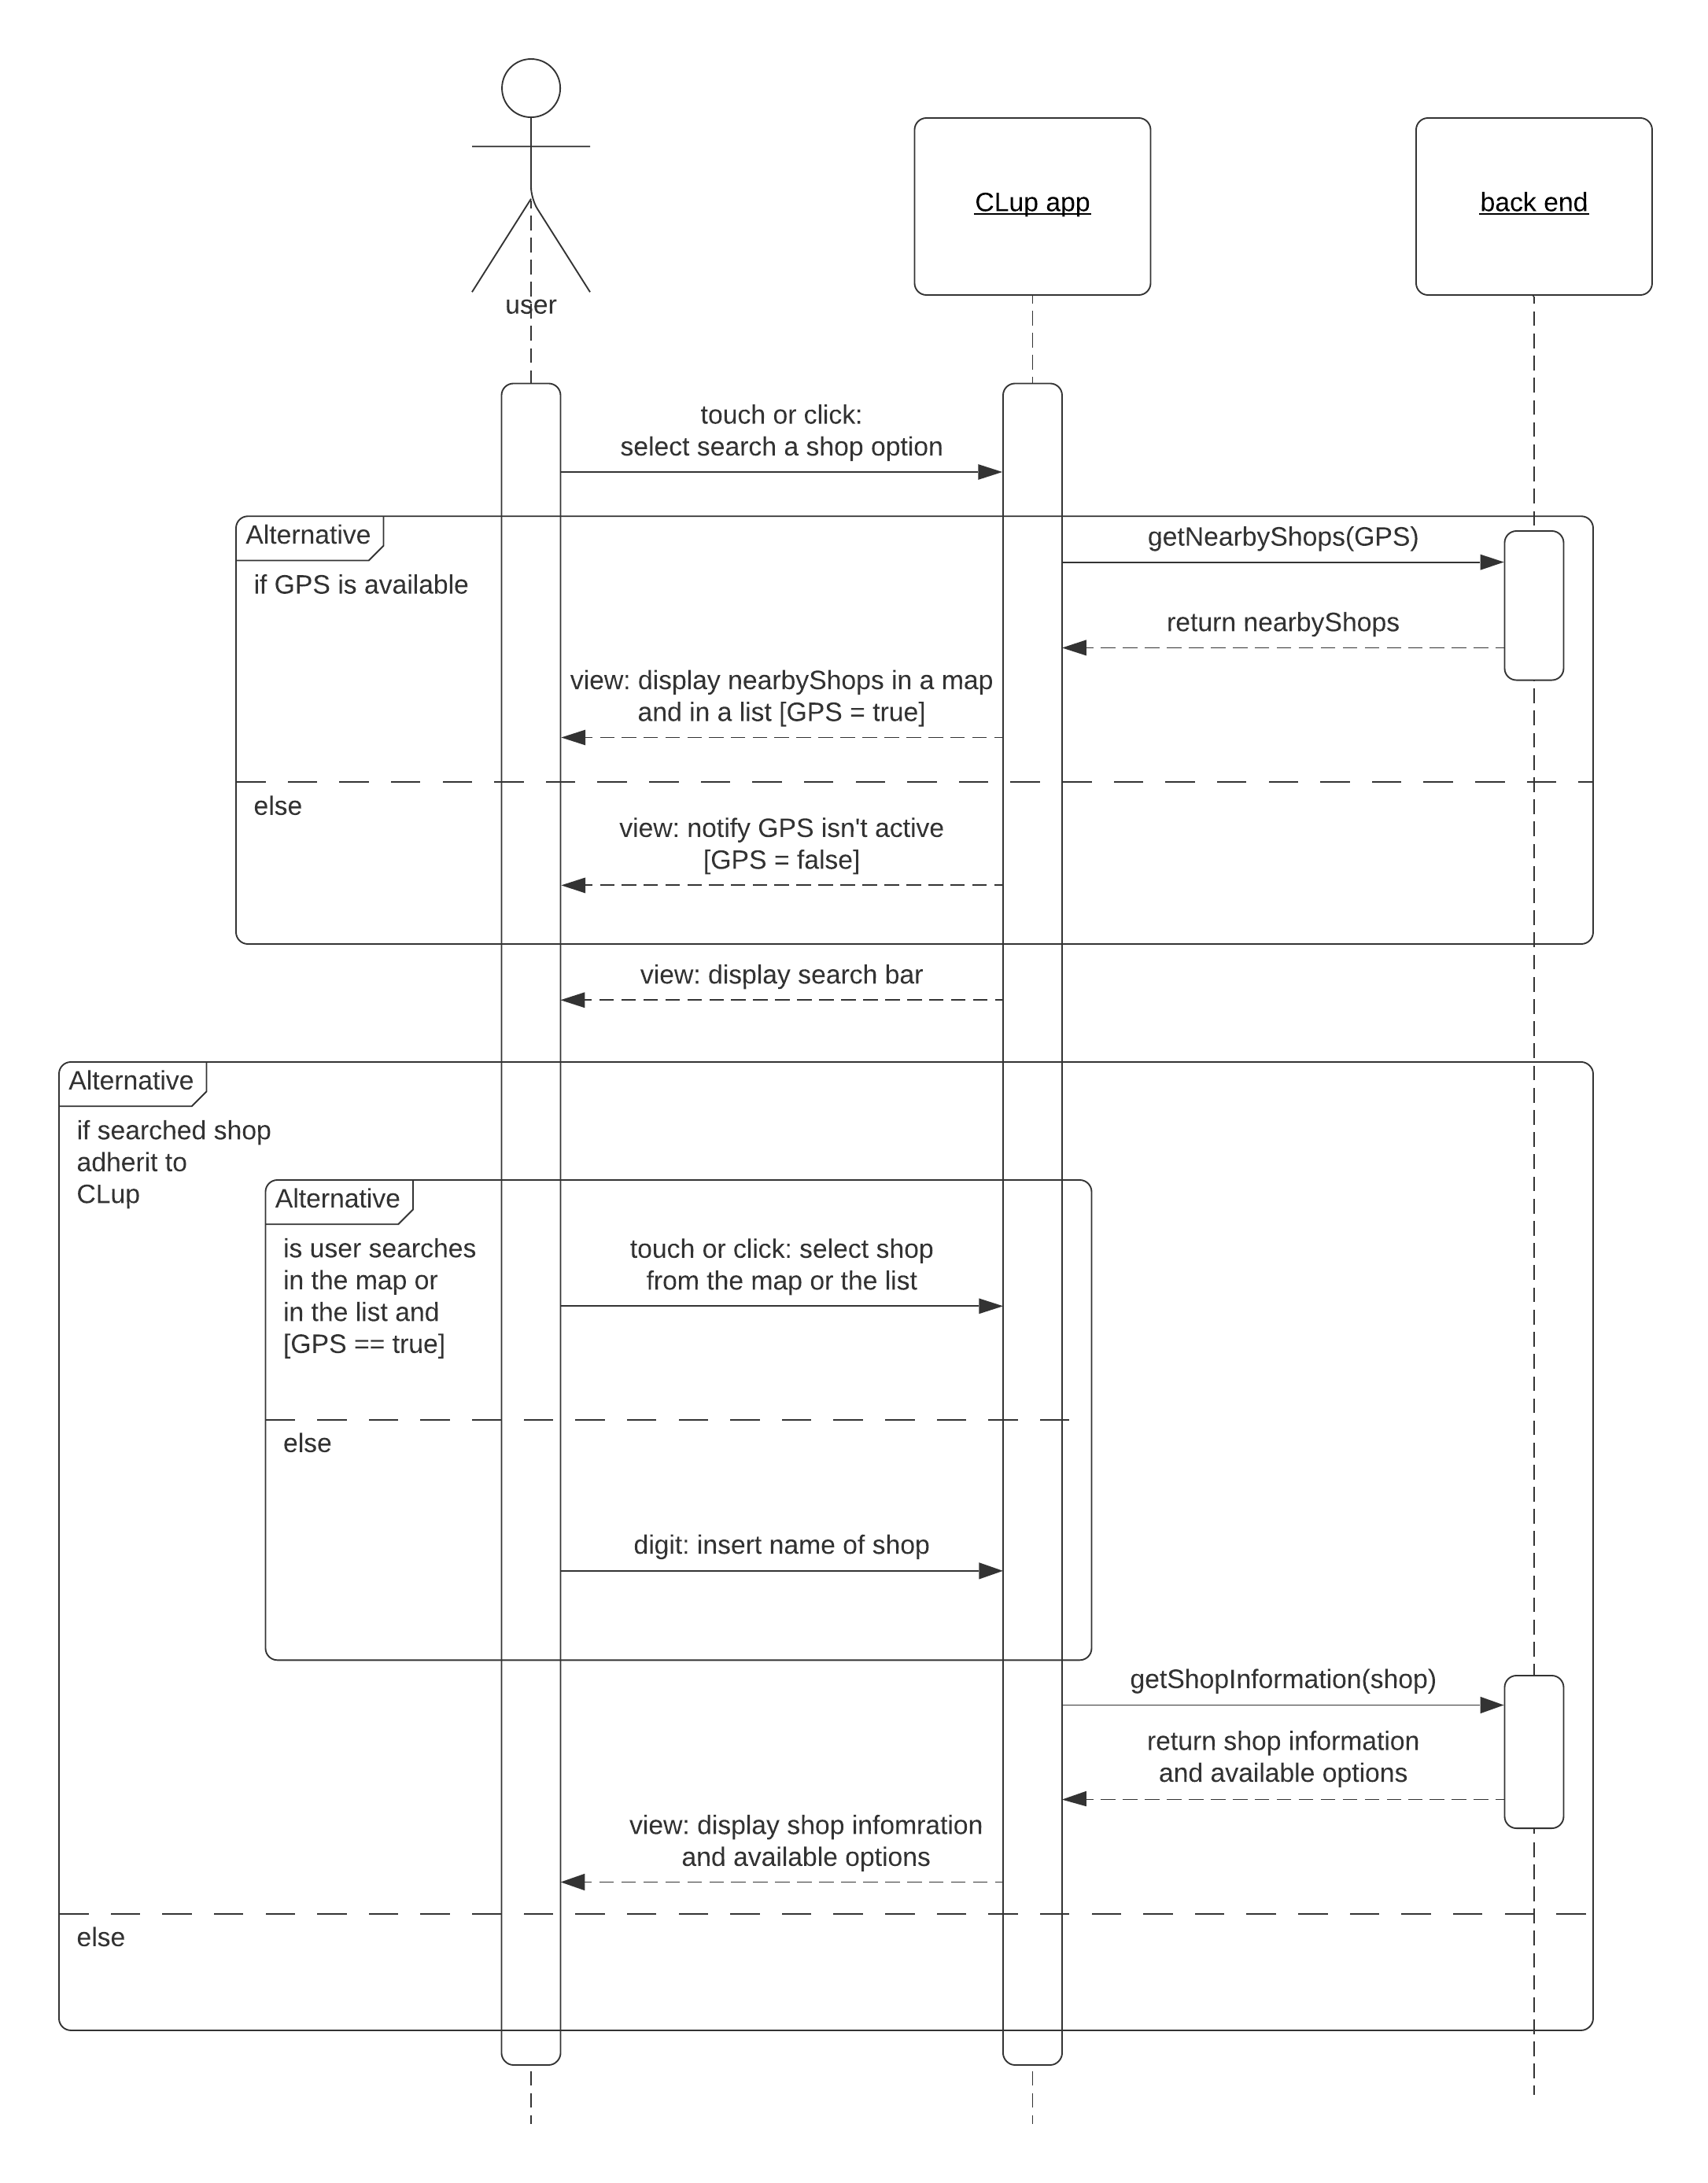
\includegraphics[width=\textwidth]{Images/Use case - user searches a shop.png}
    \caption{\label{fig:usersearchesshop}User searches a shop - sequence diagram}
\end{figure}

\clearpage
\subsection{Product perspective}
\label{subsect:productperspective}

Here we include further details on the shared phenomena and a domain model (class diagrams and statecharts).

Describes external interfaces: system, user, hardware, software; also operations and site adaptation, and hardware constraints

\subsubsection{Class diagrams and statecharts}
\label{subsubsect:diagrams}

What should we model? The objects and people that are of interest for the given problem. The relevant phenomena. The goals, requirements, and domain assumptions.

How do we find objects? Analyze any description of the problem, the application domain, the scenarios and use cases. 

to model dynamic behavior of a single object we use state machine diagram.

From the flow of events in the use case or scenario, proceed to the sequence diagram. A sequence diagram is a graphical description of objects participating in a use case or scenario using a DAG (directed acyclic graph) notation.

Consider using state diagrams and activity diagrams.

What is the structure of the world? $\rightarrow$ Create class siagrams for static information models (UML). Is there any state change in an object that is to be defined explicitly? $\rightarrow$ Create state diagrams for dynamic class behavior models. How is the expected interaction between the software to be and the environment? Create sequence diagrams from use cases for dynamic object behavior instance examples; or create activity diagrams when you want to highlight important process.

UML does not help us in expressing assertions, we can complement its usage with some formal or informal description of these assertions.

\subsection{Product functions}
\label{subsect:productfunctions}

Here we include the most important requirements.

\subsection{User characteristics}
\label{subsect:usercharacteristics}

Here we include anything that is relevant to clarify their needs.

\subsubsection{Actors}
\label{subsubsect:actors}

Customer: a person who grocery shops.
user: a customer using Clup and who is registered on the system. They can join the virtual queue, book a shopping session and ask/receive updates.
Shop manager: a person who register their shop on Clup. A shop manager can register multiple shop on the system.
Shop: a grocery shop registered on the system. It updates periodically the people present in the store and sends updates to the manager.

\subsection{Phenomena [sezione provvisoria]}
\label{subsect:phenomena}

The machine: the portion of system to be developed.
The world (a.k.a. the environment): the portion of the real-world affected by the machine.
Requirements engineering is concerned with phenomena occurring in the world, as opposed to phenomena occurring inside the machine.

Goals are prescriptive assertions formulated in terms of \textbf{world} phenomena (not necessarily shared).
Domain properties/assumptions are descriptive assertions assumed to hold in the \textbf{world}.
Requirements are prescriptive assertions formulated in terms of \textbf{shared} phenomena.
Requirements are a bridge from the \textbf{machine} to the real \textbf{world}.

Find all the possible phenomena, for each one specify if its shared or not and who controls it (world or machine). 

\subsubsection{World phenomena}
\label{subsubsect:worldphenomena}

World phenomena are phenomena that the machine can not observe.

\subsubsection{Shared Phenomena}
\label{subsubsect:sharedphenomena}

Some world phenomena are shared with the machine.
Shared phenomena can be controlled by the world and observed by the machine, or controlled by the machine andd observed by t5he world.
